\section{Simulación}\label{sec:simulacion}

\begin{frame}{Parámetros de simulación}
    \begin{block}{Parámetros fijos}
        \begin{itemize}
            \item Longitud $L = 0.1 m$
            \item Radio de las partículas $r = 0.001 m$
            \item Radio del obstáculo y partícula grande $R = 0.005 m$
            \item Masa de las partículas $m = 1 kg$
            \item Masa de la partícula grande $M = 3 kg$
        \end{itemize}
    \end{block}

    \begin{block}{Parámetros variables}
        \begin{itemize}
            \item Velocidad inicial de las partículas $v_0$
            \item Cantidad de partículas $N$
            \item Cantidad de iteraciones $I$
            \item Tiempo de simulación $T$
        \end{itemize}
    \end{block}

\end{frame}

\begin{frame}{Esquema del sistema}
    \text{Esquema simplificado con las variables de simulación.}
    \begin{figure}[H]
        \centering
        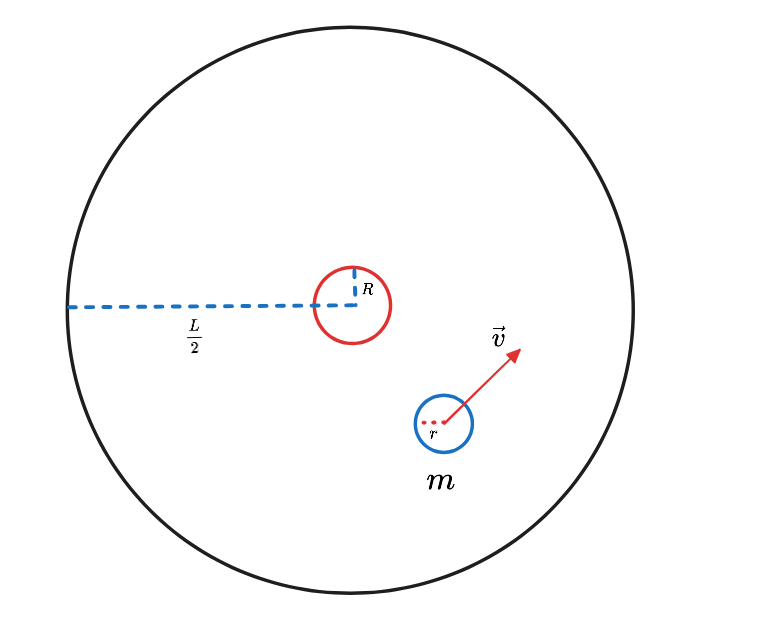
\includegraphics[width=0.4\linewidth]{pic/04-sim/system-schema}\label{fig:figure-system-schema}
    \end{figure}
\end{frame}

\begin{frame}{Observables}
    \begin{block}{Presión}
        \text{Fuerza promedio por unidad de área.}
        \begin{equation*}
            P = \frac{F^{\hat{n}}}{L} = \frac{m \sum_{i=1}^{N} v_{i}^{\hat{n}}}{L \Delta t}
        \end{equation*}
    \end{block}

    \begin{block}{Temperatura}
        \text{Proporcional a la energía cinética promedio de las partículas.}
        \begin{equation*}
            T \propto v_{i}^{2}
        \end{equation*}
    \end{block}
\end{frame}

\begin{frame}{Observables}
    \begin{block}{Tiempo promedio de colisión}
        \text{Tiempo medio en que cierto porcentaje de las partículas colisionan con el obstáculo.}
        \begin{equation*}
            \tau = \frac{1}{N} \sum_{i=1}^{N} t_i
        \end{equation*}
    \end{block}

    \begin{block}{Pendiente de colisión}
        \text{Variación en la cantidad de colisiones con el obstáculo en función del tiempo.}
        \begin{equation*}
            m = \frac{dCol}{dt}
        \end{equation*}
    \end{block}
\end{frame}

\begin{frame}{Observables}
    \begin{block}{Desplazamiento cuadrático medio}
        \begin{minipage}[t]{0.7\linewidth}
            \text{Promedio de la distancia que recorre la partícula grande al cuadrado.}
            \begin{equation*}
                \langle z^2 \rangle = 2 D t
            \end{equation*}
        \end{minipage}%
        \hfill%
        \begin{minipage}[t]{0.2\linewidth}
            \begin{figure}[H]
                \centering
                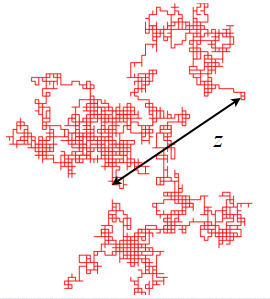
\includegraphics[width=0.5\linewidth]{pic/04-sim/dcm}\label{fig:figure-dcm}
            \end{figure}
        \end{minipage}
    \end{block}

    \begin{block}{Fórmula de error}
        \text{Utilizado para ajustar el coeficiente de difusión $D$.}
        \begin{equation*}
            E(D) = \sum (y_i - f(x_i, D))^2
        \end{equation*}
    \end{block}
\end{frame}





